\subsection{Lab8: Receptor FM monofónico}
%*********************
\begin{frame}{}

\pgfdeclareimage[width=\paperwidth,height=\paperheight]{bg}{imagenes/fondo_lab}
\setbeamertemplate{background}{\pgfuseimage{bg}}

\bfseries{\textrm{\LARGE Lab8\\ \Large Receptor FM monofónico}}
\raggedright
\end{frame}
%*********************



\begin{frame}{Receptor FM monofónico}

\pgfdeclareimage[width=\paperwidth,height=\paperheight]{bg}{imagenes/fondo3}
\setbeamertemplate{background}{\pgfuseimage{bg}}


En este laboratorio, se realizará la simulación de un receptor FM monofónico en el cual se muestra la función de cada uno de los bloques que conforma dicho receptor, además se muestra el proceso matemático para llegar a 48 KHz de la tasa de muestreo que se va a establecer.



\end{frame}
%---------------------------------

\begin{frame}{Modulación de frecuencia}

Se refiere a la forma de transmitir información a través de una Onda portadora variando su frecuencia. En este tipo de modulación la variación se produce en los saltos de frecuencias. \\ \vspace{2mm}

La modulación de frecuencia se usa comúnmente en las radiofrecuencias de muy alta frecuencia por la alta fidelidad de la radiodifusión de la música y el habla. El sonido de la televisión analógica también se difunde por medio de FM. \\ \vspace{2mm}

La modulación de frecuencia también se utiliza en las frecuencias de audio para sintetizar sonido. Está técnica, conocida como síntesis FM, fue popularizada a principios de los sintetizadores digitales y se convirtió en una característica estándar para varias generaciones de tarjetas de sonido de computadoras personales.

\end{frame}
%---------------------------------


\begin{frame}{Modulación de frecuencia}

\textbf{Aplicaciones en radio}

Dentro de las aplicaciones de FM se encuentra la radio, donde los receptores emplean un detector de FM y el sintonizador es capaz de recibir la señal más fuerte de las que transmiten en la misma frecuencia. Otra de las características que presenta FM es la de poder transmitir señales estereofónicas. \\ \vspace{2mm}

\textbf{Otras aplicaciones}

Entre otras de sus aplicaciones se encuentran la televisión, SECAM: El sistema de televisión en color SECAM modula la información de color en FM. como sub-portadora de sonido; en micrófonos inalámbricos; y como ayuda en navegación aérea, En los sistemas de vídeo analógicos, incluyendo VHS, para registrar la luminancia (blanco y negro) de la señal de video\cite{Wikipedia8}.\\ \vspace{2mm}


\end{frame}
%---------------------------------

\begin{frame}{Diagrama del receptor FM monofónico}

\begin{figure}[H]
\centering
\vspace{-3mm}
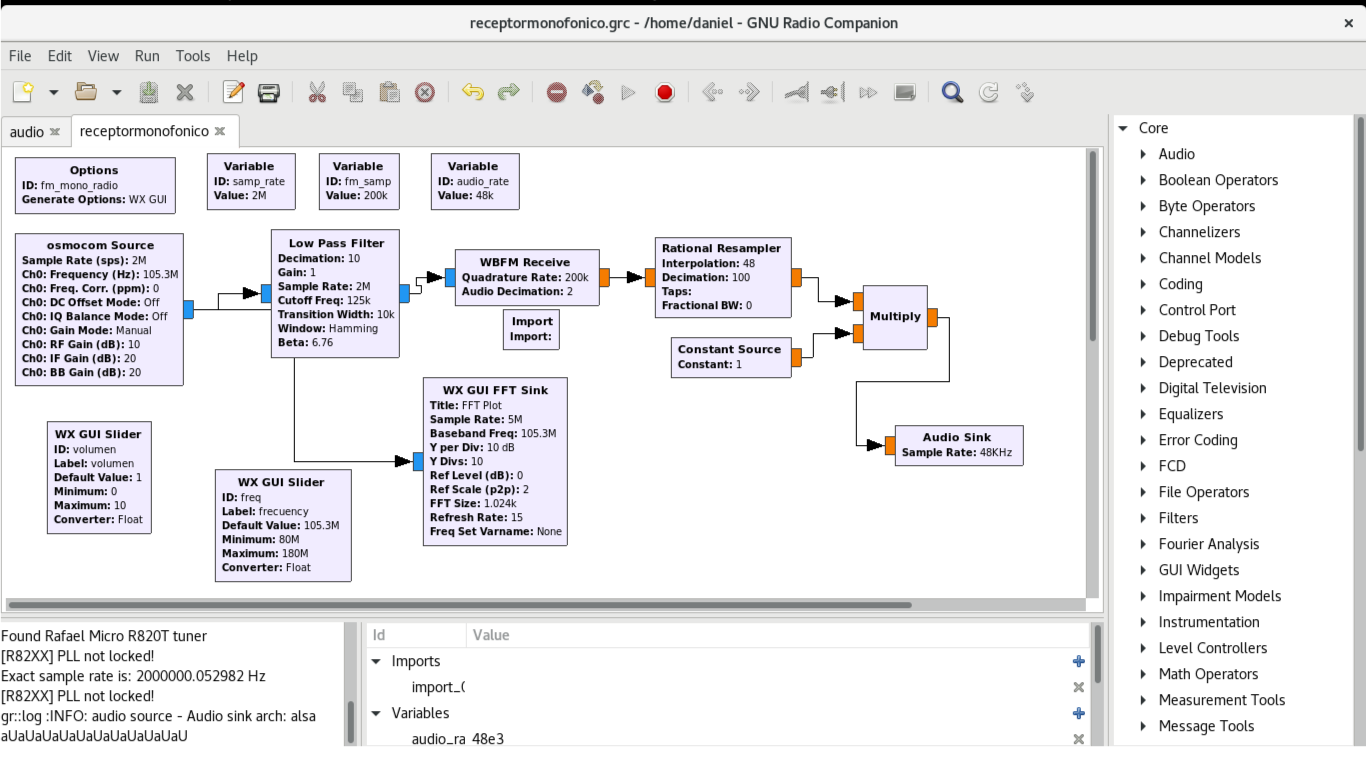
\includegraphics[width=\textwidth]{parte3/lab8/pdf/lab8_1.pdf}
\end{figure}

\end{frame}
%---------------------------------

\begin{frame}{Receptor FM monofónico}

\begin{figure}[H]
\centering
\vspace{-3mm}
\includegraphics[width=\textwidth]{parte3/lab8/pdf/lab8_2.pdf}
\end{figure}

\end{frame}
%---------------------------------

\begin{frame}{Receptor FM monofónico}

\begin{figure}[H]
\centering
\vspace{-3mm}
\includegraphics[width=\textwidth]{parte3/lab8/pdf/lab8_3.pdf}
\end{figure}

\end{frame}
%---------------------------------

\begin{frame}{Receptor FM monofónico}

\begin{figure}[H]
\centering
\vspace{-3mm}
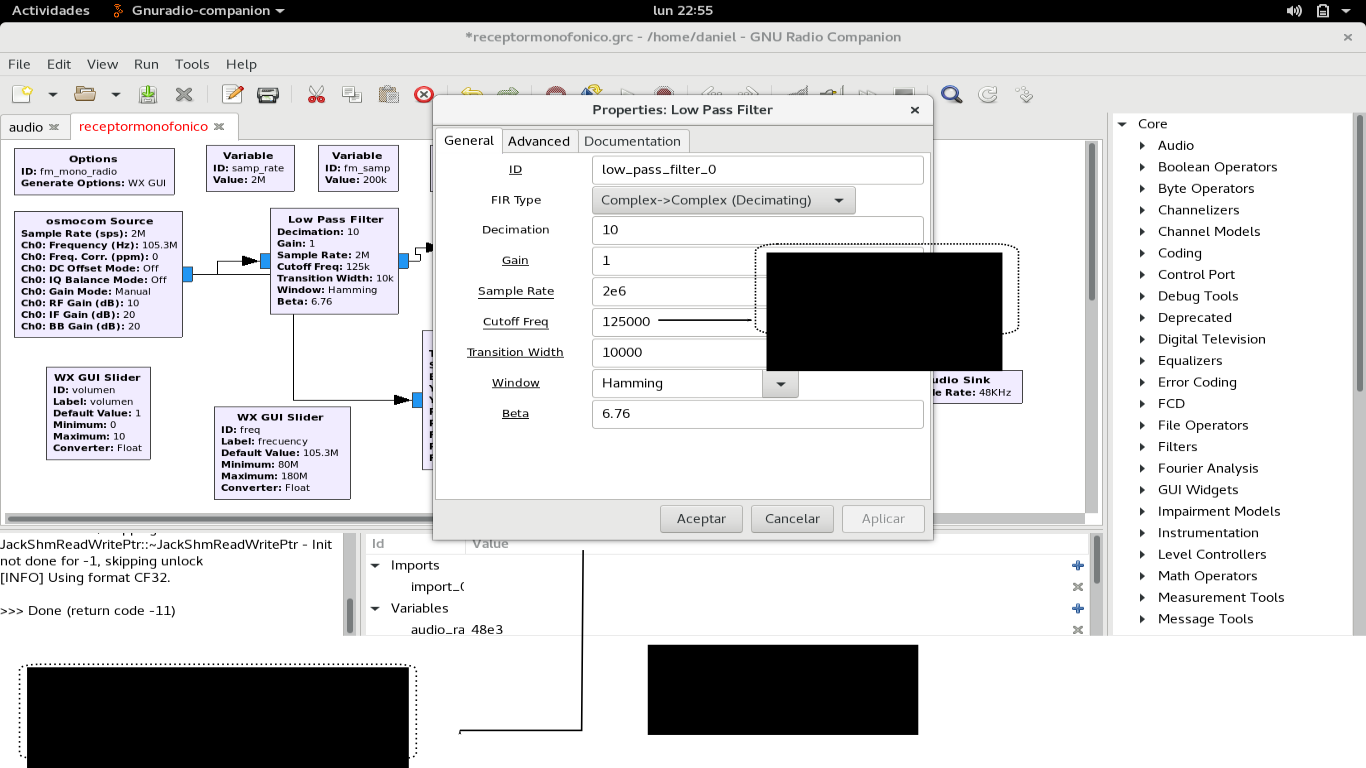
\includegraphics[width=\textwidth]{parte3/lab8/pdf/lab8_4.pdf}
\end{figure}

\end{frame}
%---------------------------------

\begin{frame}{Receptor FM monofónico}

\begin{figure}[H]
\centering
\vspace{-3mm}
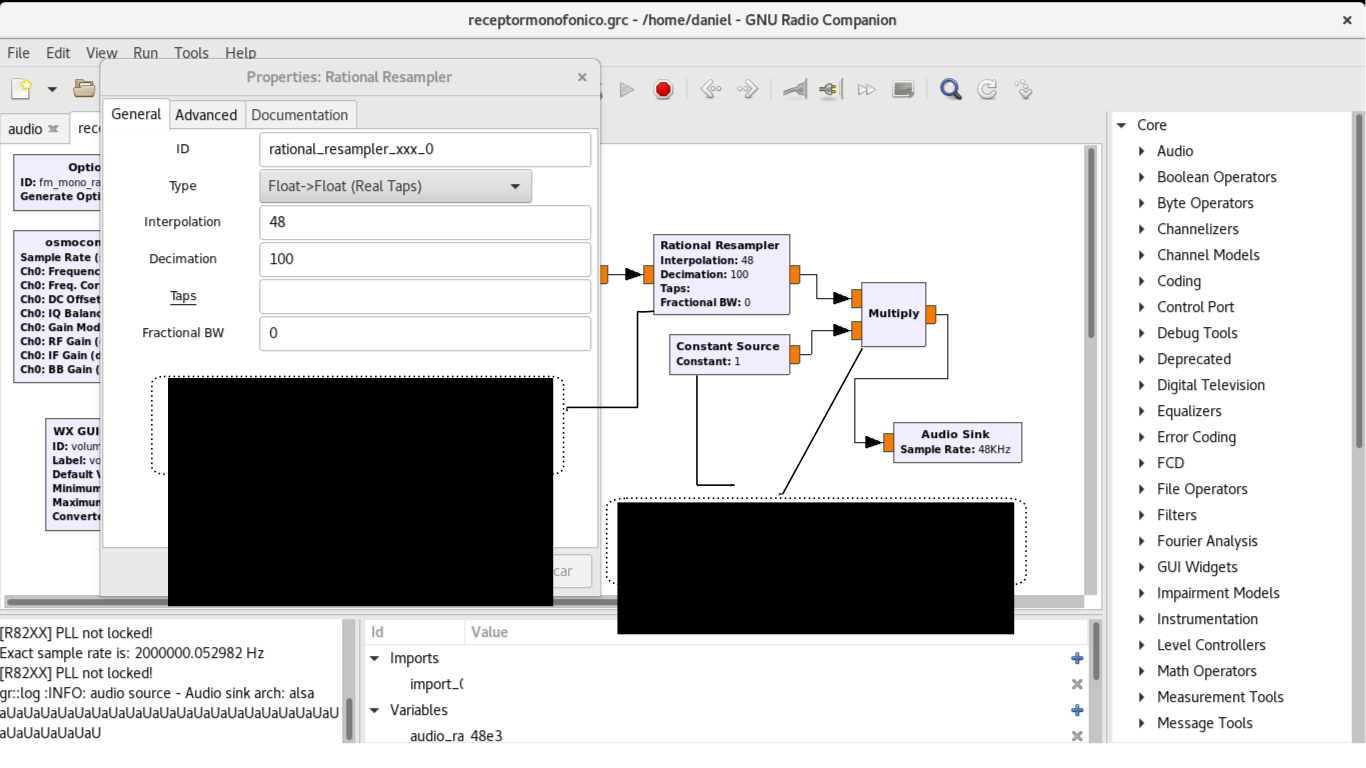
\includegraphics[width=\textwidth]{parte3/lab8/pdf/lab8_5.pdf}
\end{figure}

\end{frame}
%---------------------------------

\begin{frame}{Receptor FM monofónico}

\begin{figure}[H]
\centering
\vspace{-3mm}
\includegraphics[width=\textwidth]{parte3/lab8/pdf/lab8_6.pdf}
\end{figure}

\end{frame}
%---------------------------------

\begin{frame}{Proceso matemático}

\begin{figure}[H]
\centering
\vspace{-3mm}
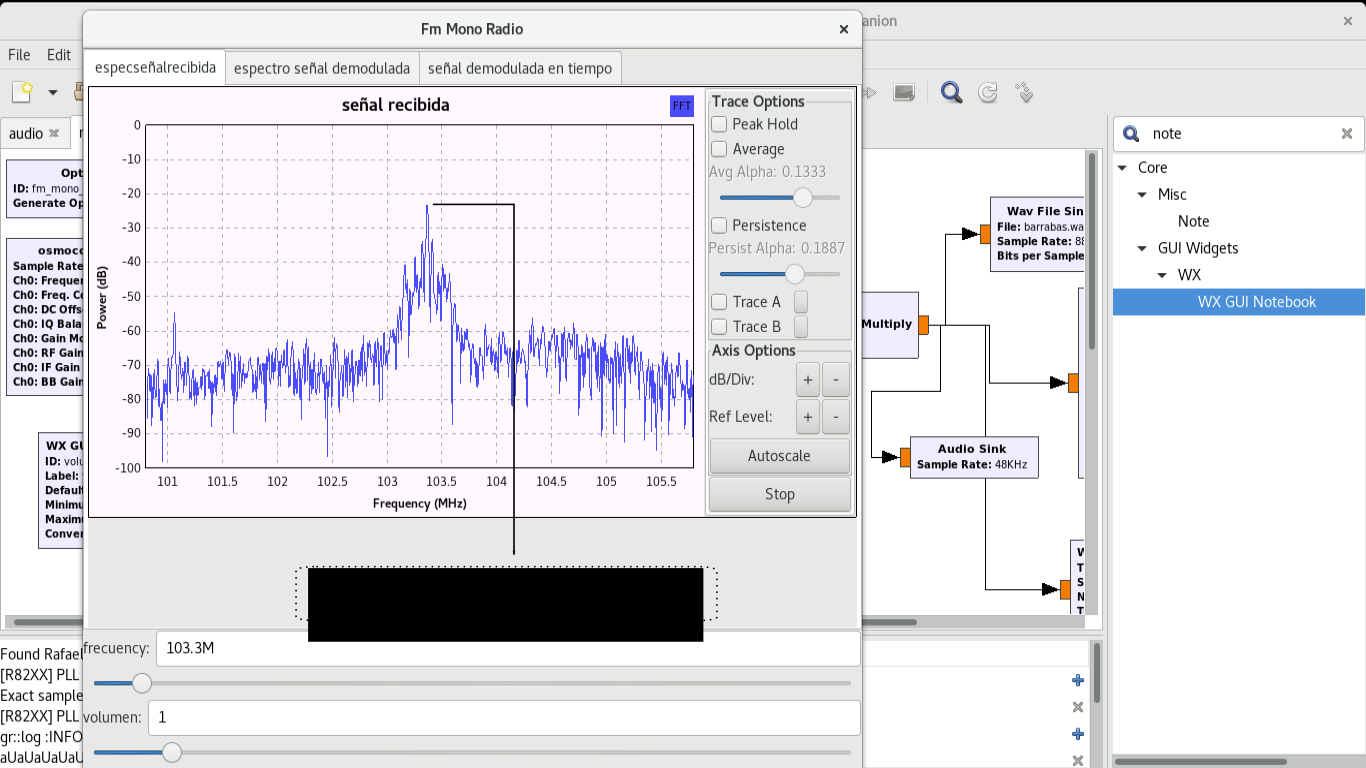
\includegraphics[width=\textwidth]{parte3/lab8/pdf/lab8_7.pdf}
\end{figure}

\end{frame}
%---------------------------------

\begin{frame}{Receptor FM monofónico}

\begin{figure}[H]
\centering
\vspace{-3mm}
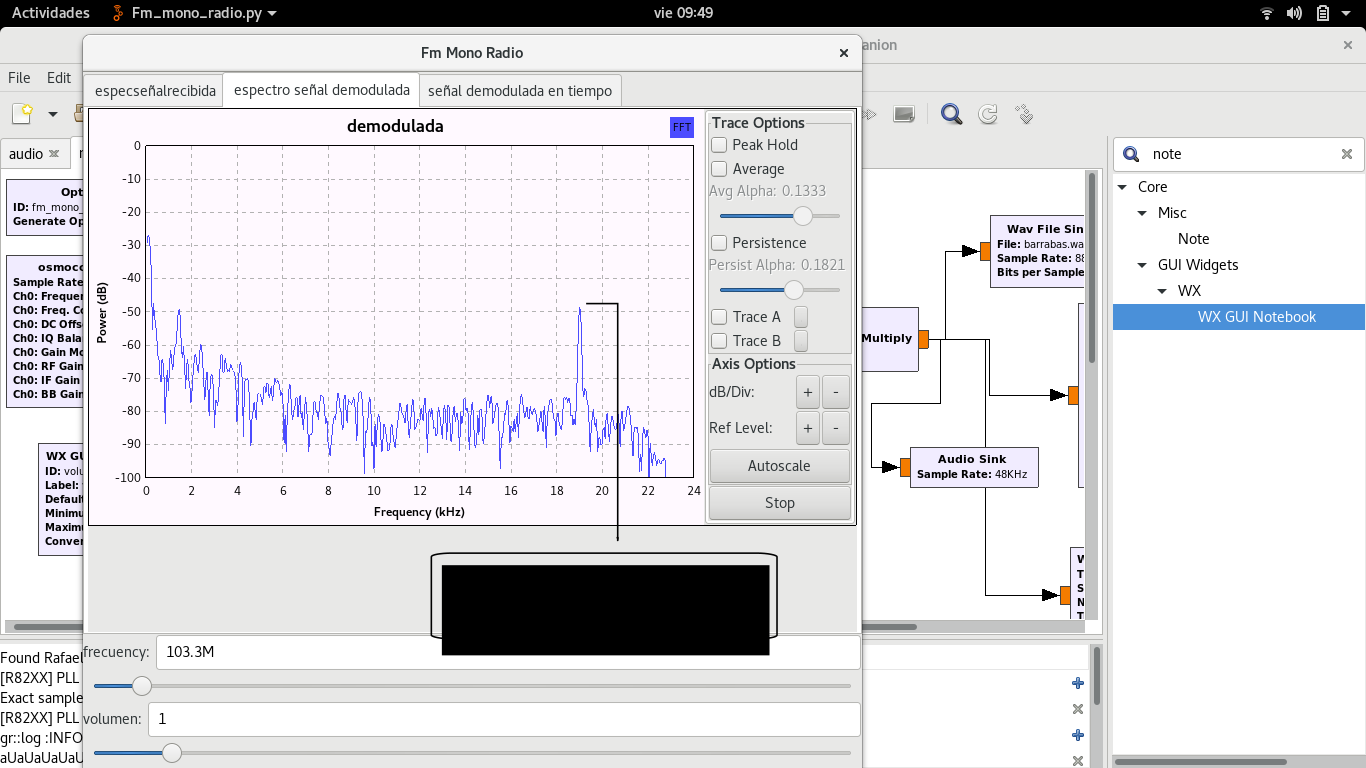
\includegraphics[width=\textwidth]{parte3/lab8/pdf/lab8_8.pdf}
\end{figure}

\end{frame}
%---------------------------------

\begin{frame}{Espectro señal recibida}

\begin{figure}[H]
\centering
\vspace{-3mm}
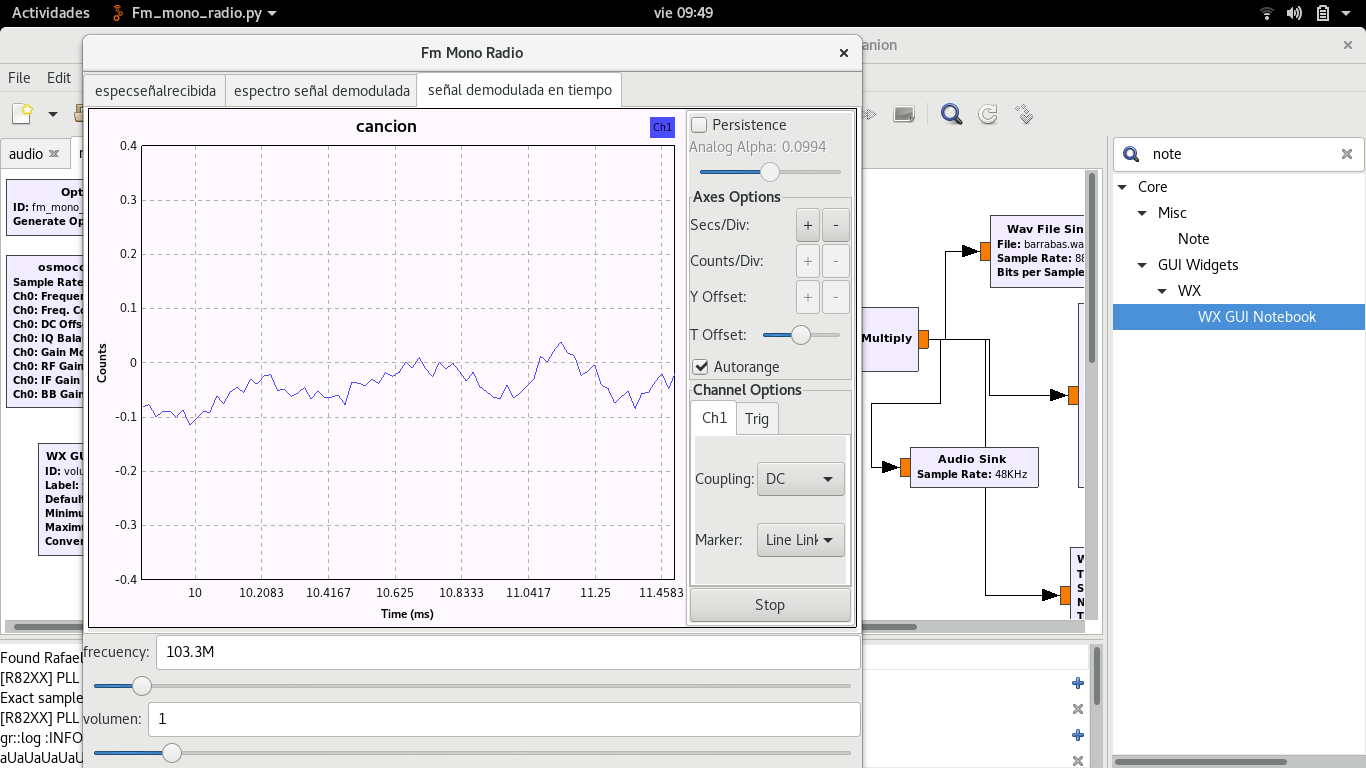
\includegraphics[width=\textwidth]{parte3/lab8/pdf/lab8_9.pdf}
\end{figure}

\end{frame}
%---------------------------------


\begin{frame}{Espectro señal demodulada}

\begin{figure}[H]
\centering
\vspace{-3mm}
\includegraphics[width=\textwidth]{parte3/lab8/pdf/lab8_10.pdf}
\end{figure}

\end{frame}
%---------------------------------


\begin{frame}{Señal demodulada en el tiempo}

\begin{figure}[H]
\centering
\vspace{-3mm}
\includegraphics[width=\textwidth]{parte3/lab8/pdf/lab8_11.pdf}
\end{figure}

\end{frame}
%---------------------------------
